\documentclass{beamer}
\usetheme{metropolis}
\usepackage{graphicx}
\usepackage{amsmath}
\title{A History of Science in Latin America (INTD290): Unit 2}
\author{Jordan Hanson}
\institute{Whittier College Department of Physics and Astronomy}

\begin{document}
\maketitle

\section{Introduction: Gamma Ray Astrophysics}

\begin{frame}{Introduction: Gamma Ray Astrophysics}
\begin{enumerate}
\item \textbf{What is a high-energy gamma ray?}
\begin{itemize}
\item Units of energy
\item Types of particles
\item Air showers
\item Astrophysical sources
\end{itemize}
\item \textbf{How do we detect them?}
\begin{itemize}
\item The Cherenkov effect in water
\item Water-based detectors and photo-multiplier tubes (PMTs)
\end{itemize}
\item \textbf{Who detects them?}
\begin{itemize}
\item International collaborations of scientists
\item Detectors located in New Mexico, Mexico, and Chile
\end{itemize}
\end{enumerate}
\end{frame}

\section{Energy units, Particle types, Air Showers, Astrophysical Sources}

\begin{frame}{Introduction: Gamma Ray Astrophysics}
\begin{enumerate}
\item \textbf{What is a high-energy gamma ray?}
\begin{itemize}
\item Units of energy
\begin{itemize}
\item Units: electron-Volts ($1.6 \times 10^{-19}$ J), GeV, TeV, ...
\item Flux: particles per unit area, time, 2D angle on sky, ...
\end{itemize}
\item Types of particles
\begin{itemize}
\item Gamma rays: $\gamma$-ray (photon with energy greater than 1 MeV)
\item Electrons: $e^{-}$ (negative charge, mass is 511 keV)
\item Positrons: $e^{+}$ (positive charge, mass is 511 keV)
\item Muons: $\mu^{\pm}$ (negative or positive, mass is 0.106 GeV)
\item Neutrinos: $\nu$ (neutral, basically massless)
\end{itemize}
\item Air showers
\item Astrophysical sources
\end{itemize}
\end{enumerate}
\end{frame}

\begin{frame}{Introduction: Gamma Ray Astrophysics}
\small
\begin{enumerate}
\item \textbf{Air showers} - High energy particles hit the atmosphere and make other particles.
\item Astrophysical sources
\end{enumerate}

\begin{figure}
\centering
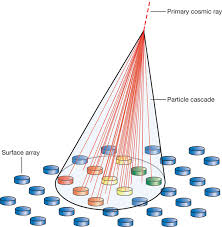
\includegraphics[width=0.45\textwidth]{figures/air_shower_1.jpeg}
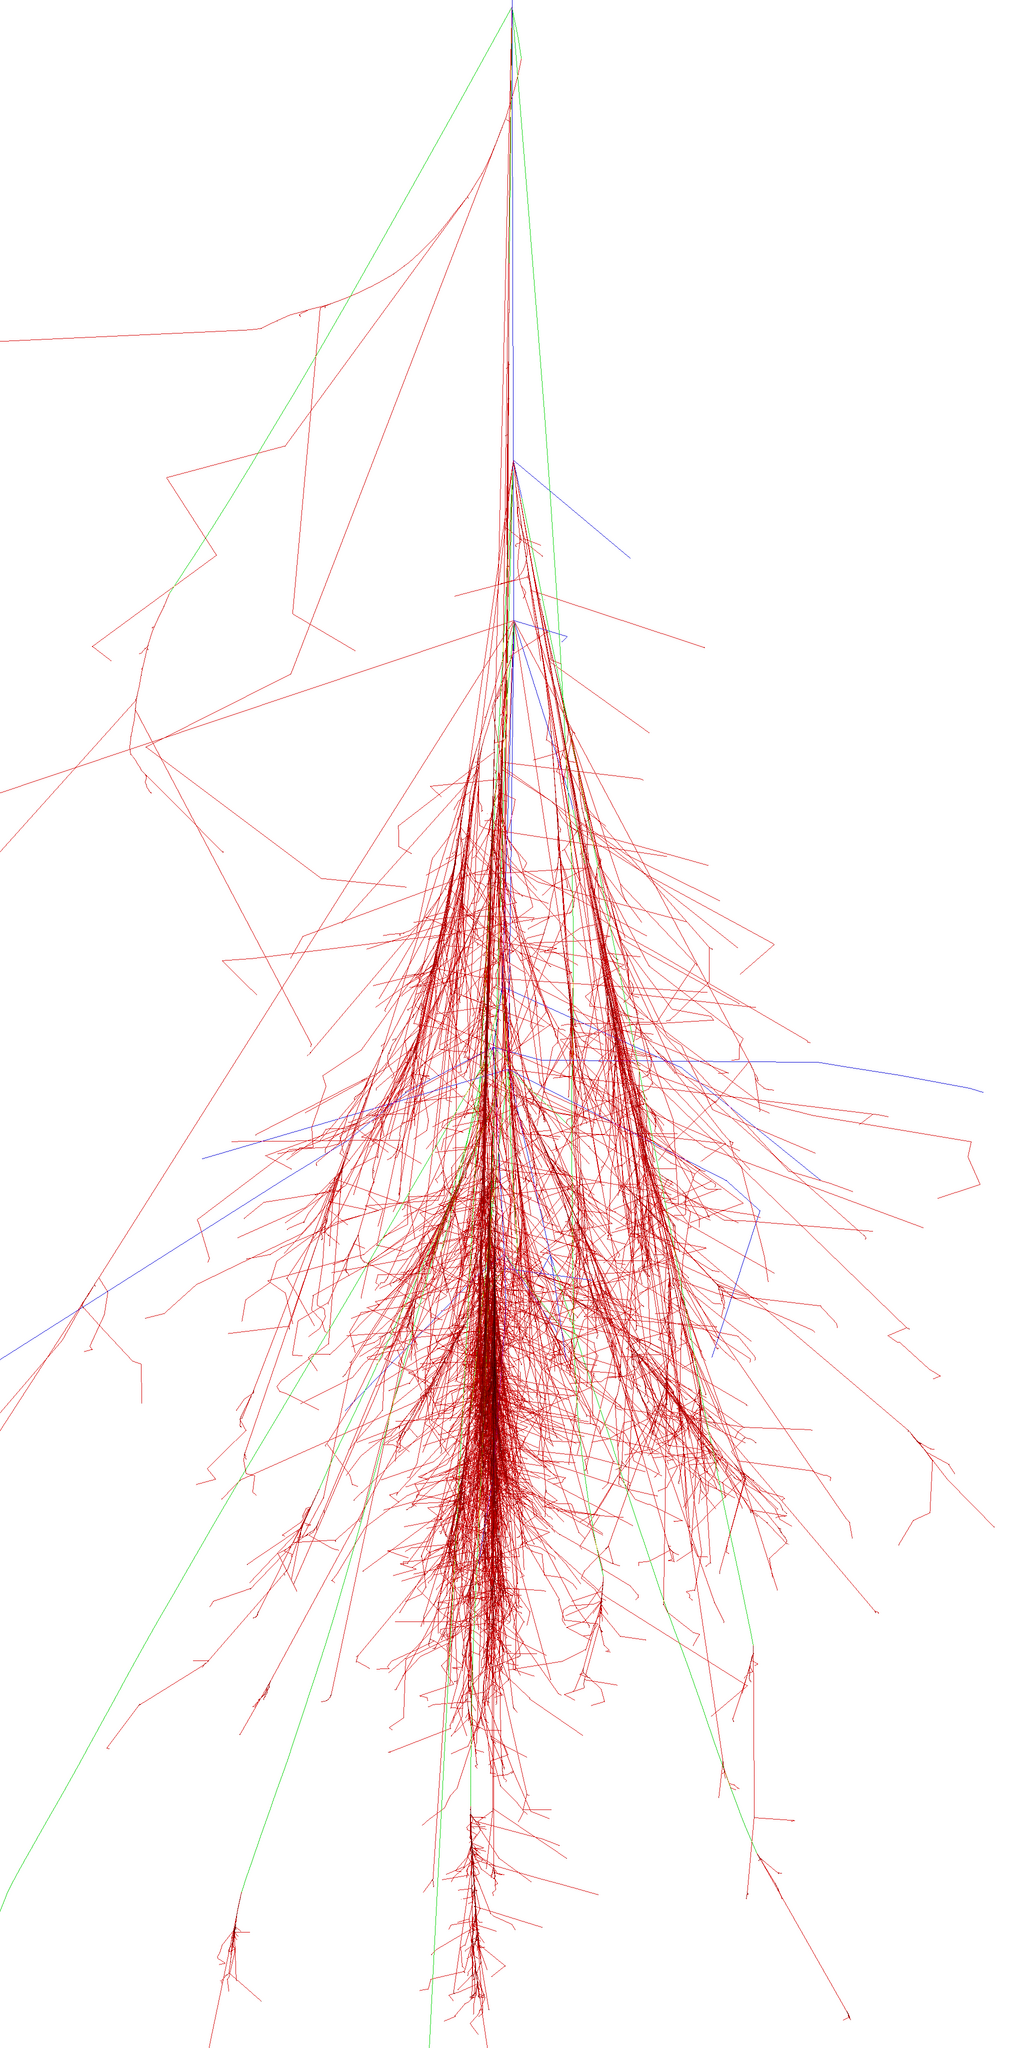
\includegraphics[width=0.2\textwidth]{figures/air_shower_2.png}
\caption{\label{fig:1} High-energy particles hit the atmosphere.}
\end{figure}
\end{frame}

\begin{frame}{Introduction: Gamma Ray Astrophysics}
\small
\begin{enumerate}
\item Air showers
\item \textbf{Astrophysical sources} ...
\end{enumerate}

\textbf{\alert{What do we put here ...}}

\end{frame}

\begin{frame}{Introduction: Gamma Ray Astrophysics: All}
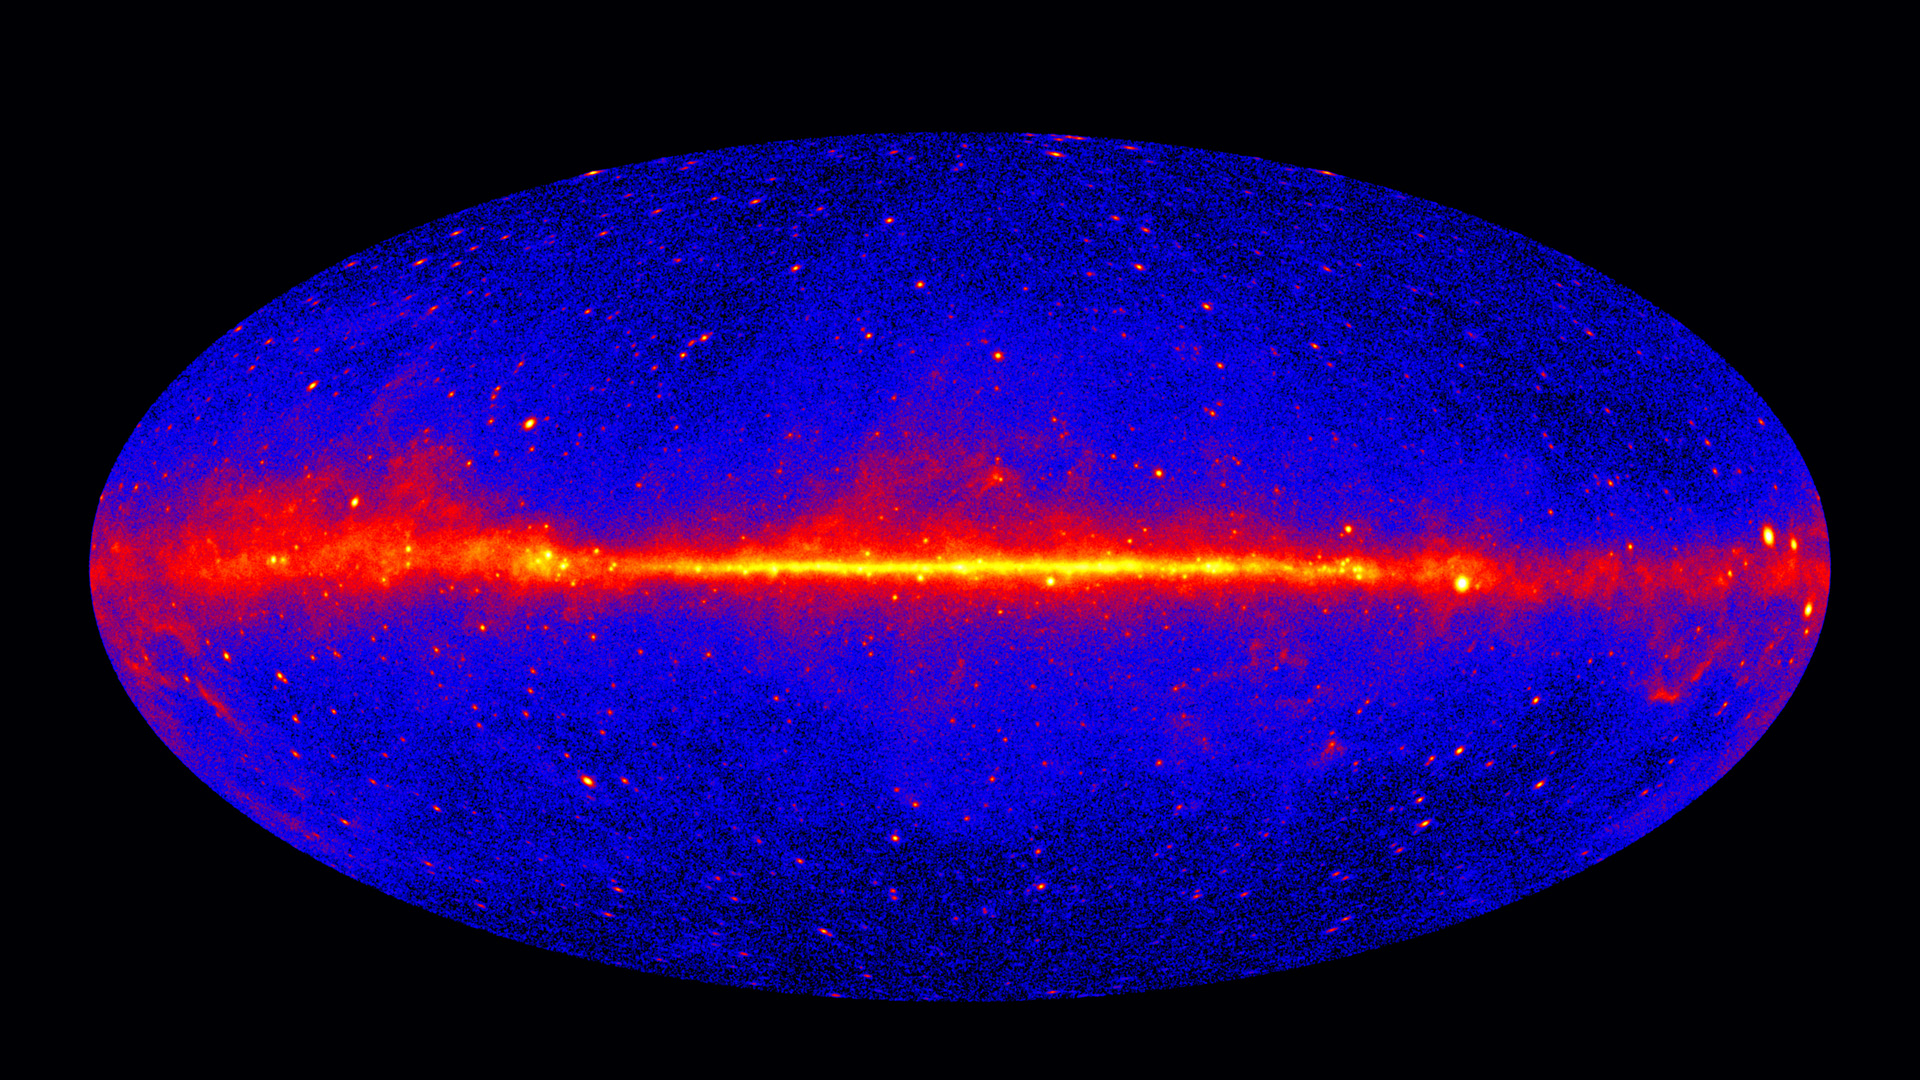
\includegraphics[width=\textwidth]{figures/all-1920.jpg}
\end{frame}

\begin{frame}{Introduction: Gamma Ray Astrophysics: Supernova}
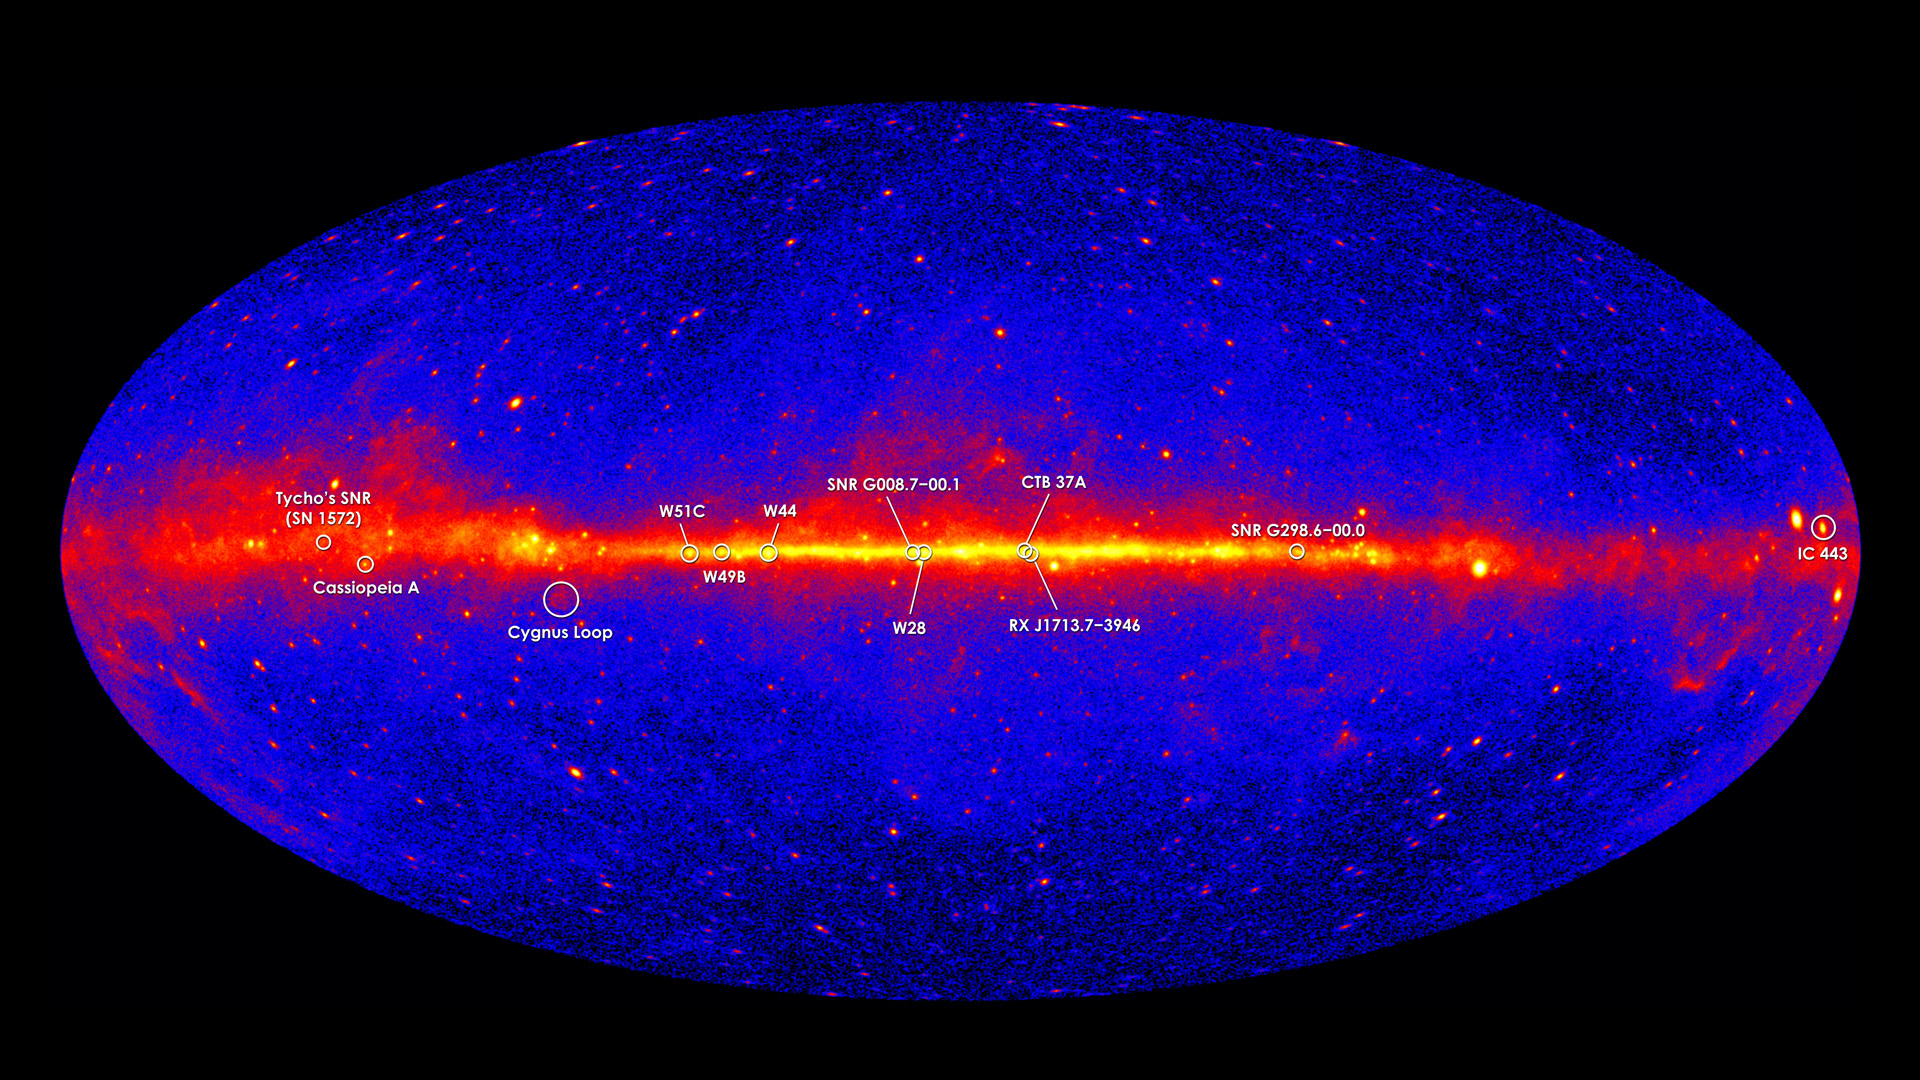
\includegraphics[width=\textwidth]{figures/superNova-1920.jpg}
\end{frame}

\begin{frame}{Introduction: Gamma Ray Astrophysics: Pulsars}
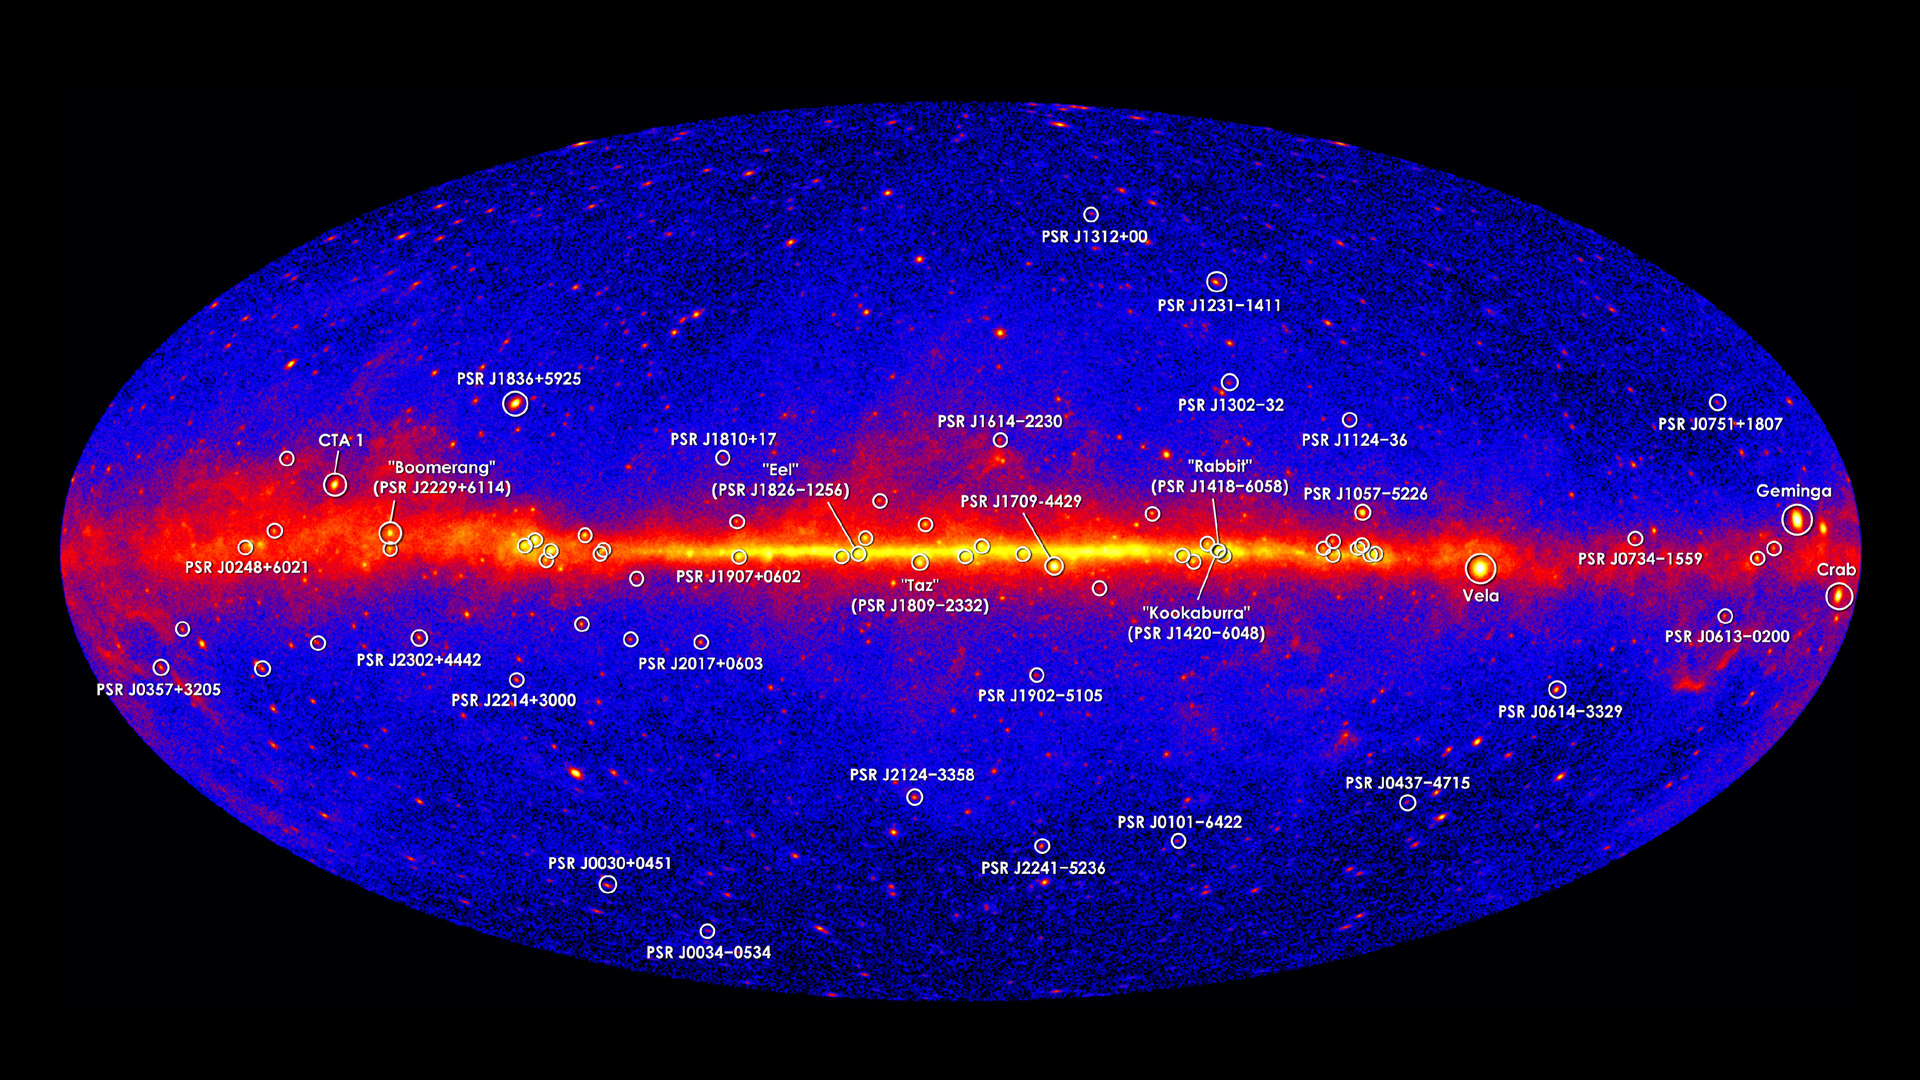
\includegraphics[width=\textwidth]{figures/pulsars-1920.jpg}
\end{frame}

\begin{frame}{Introduction: Gamma Ray Astrophysics: Black Holes}
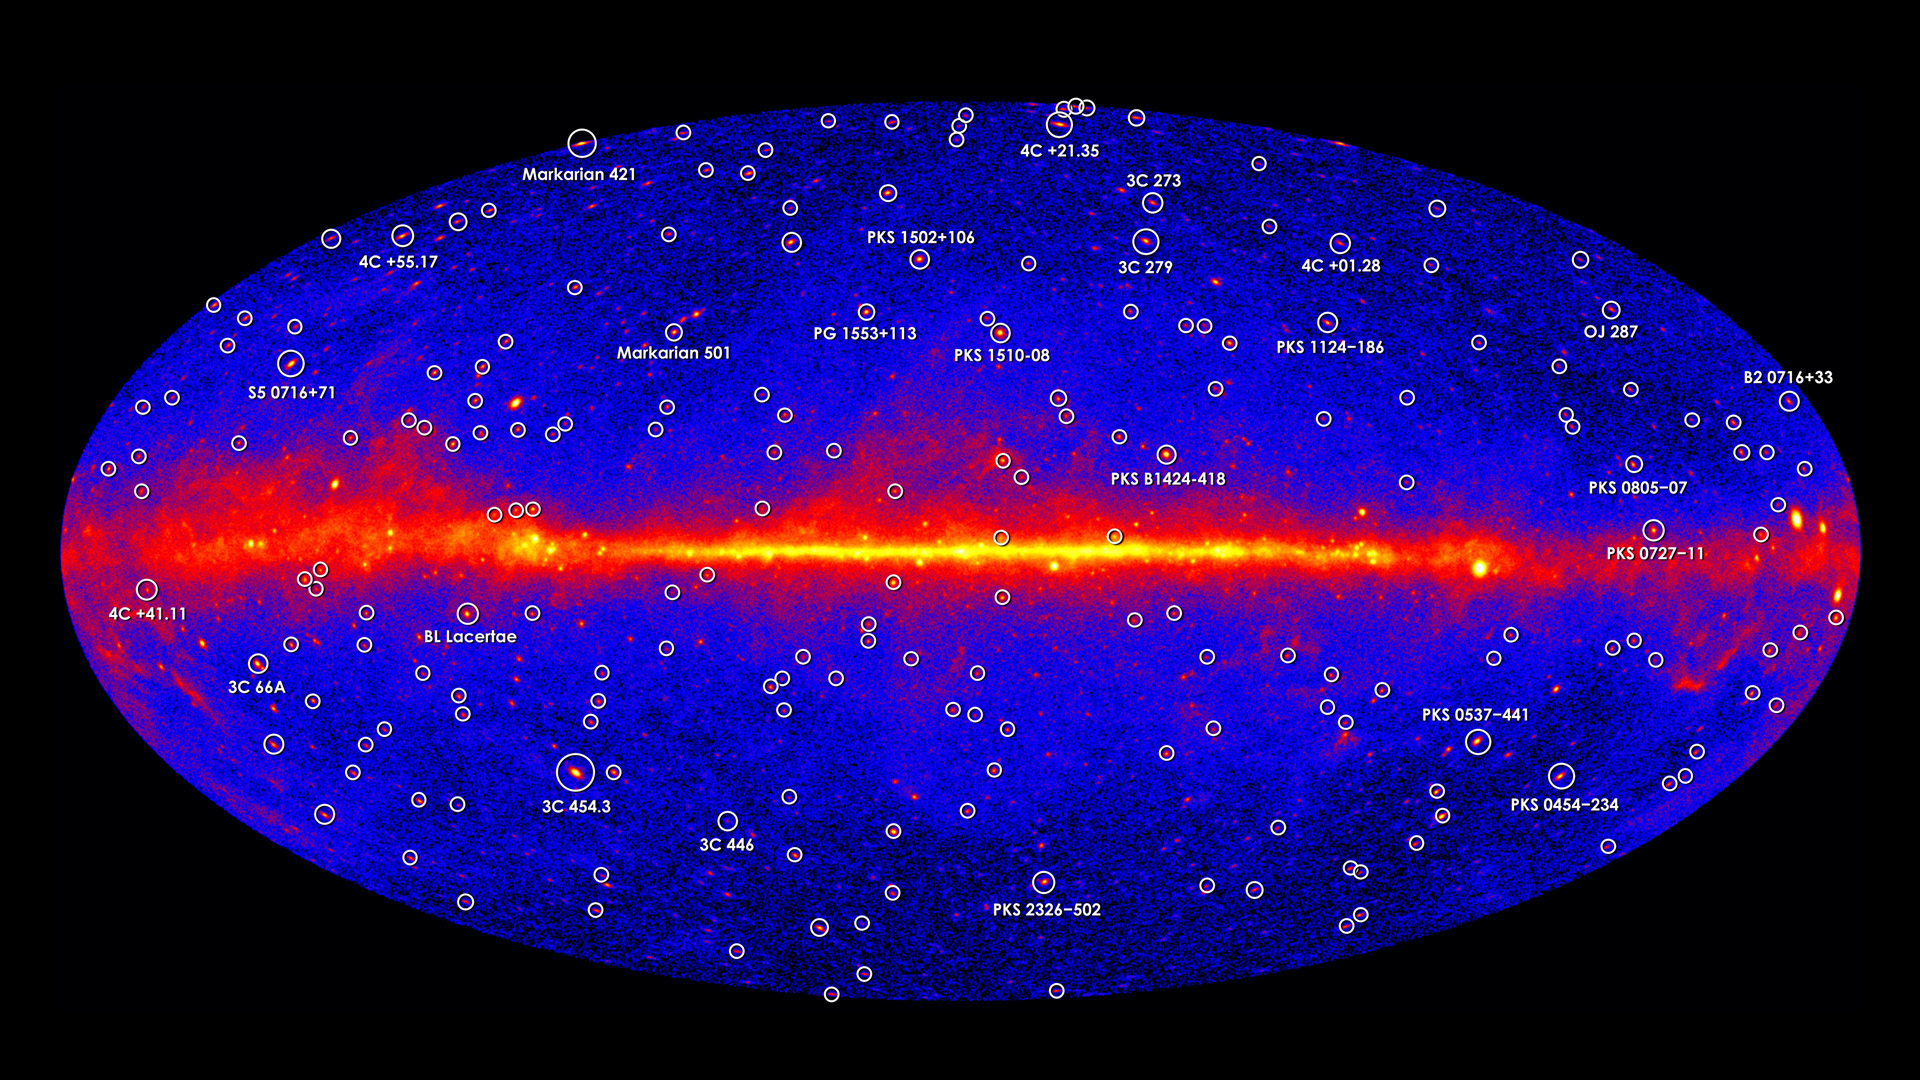
\includegraphics[width=\textwidth]{figures/blackHole-1920.jpg}
\end{frame}

\section{How do we detect them?}

\begin{frame}{How we detect them: Water-based Cherenkov Radiation}
\centering
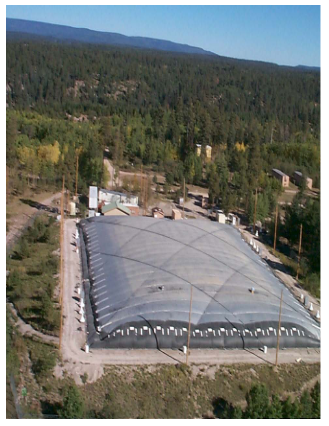
\includegraphics[width=0.3\textwidth]{figures/milagro_4.png}
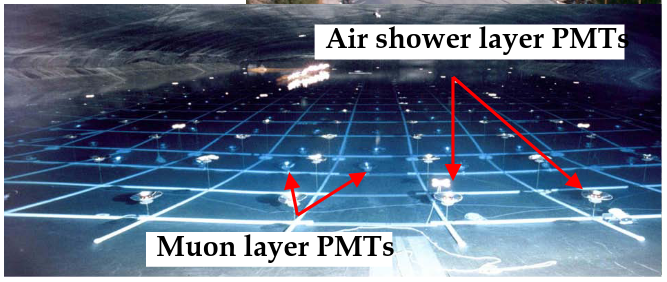
\includegraphics[width=0.45\textwidth]{figures/milagro_5.png}\\
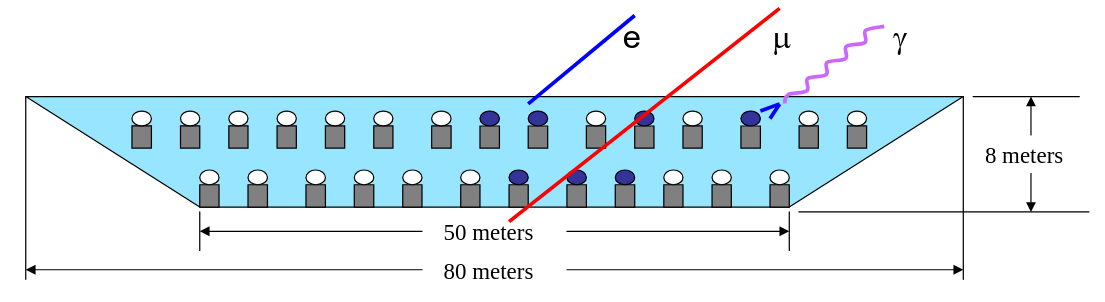
\includegraphics[width=0.95\textwidth]{figures/milagro_7.png}
\end{frame}

\begin{frame}{How we detect them: Water-based Cherenkov Radiation}
\centering
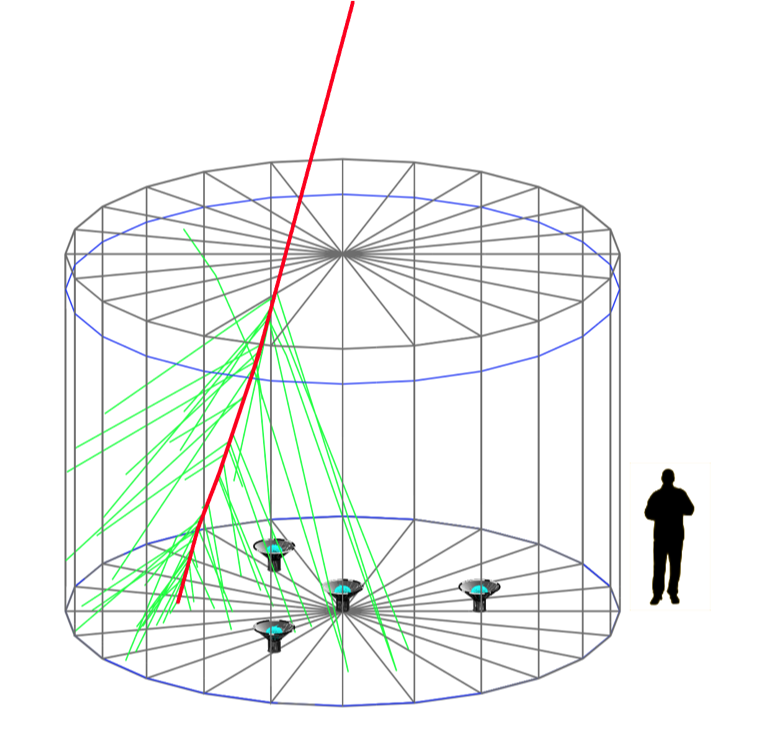
\includegraphics[width=0.45\textwidth]{figures/hawc_3.png}
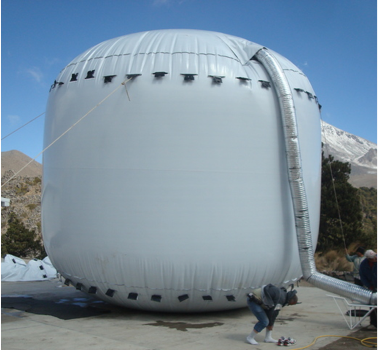
\includegraphics[width=0.45\textwidth]{figures/hawc_4.png}
\end{frame}

\section{Who detects them?}

\begin{frame}{Who detects them?}
\begin{figure}
\centering
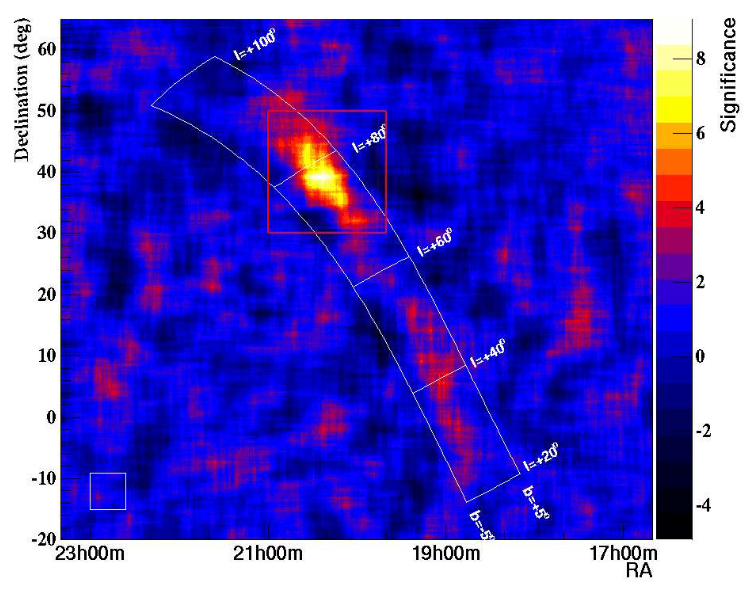
\includegraphics[width=0.8\textwidth]{figures/milagro_1.png}
\caption{\label{fig:x1} Milagro: a gamma-ray observatory in Los Alamos, NM.  Pictured: Cygnus Region.}
\end{figure}
\end{frame}

\begin{frame}{Who detects them?}
\begin{figure}
\centering
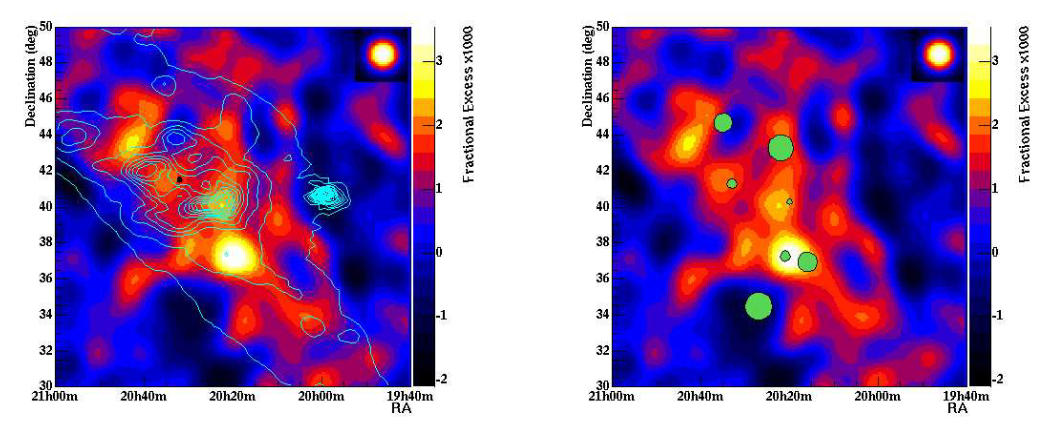
\includegraphics[width=0.8\textwidth]{figures/milagro_2.png}
\caption{\label{fig:x2} Milagro: a gamma-ray observatory in Los Alamos, NM.  Pictured: Cygnus Region.}
\end{figure}
\end{frame}

\begin{frame}{Who detects them?}
\begin{figure}
\centering
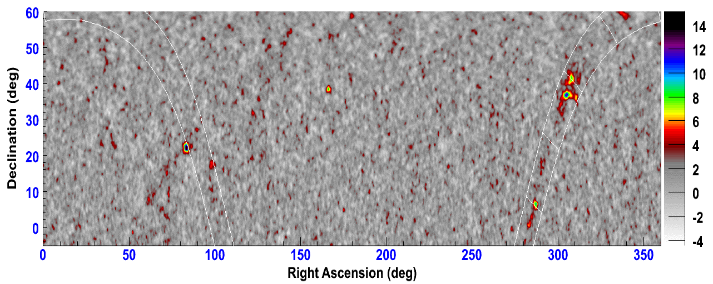
\includegraphics[width=0.8\textwidth]{figures/milagro_3.png}
\caption{\label{fig:x3} Milagro: a gamma-ray observatory in Los Alamos, NM.  Pictured: Cygnus Region.}
\end{figure}
\end{frame}

\begin{frame}{Who detects them?}
\begin{figure}
\centering
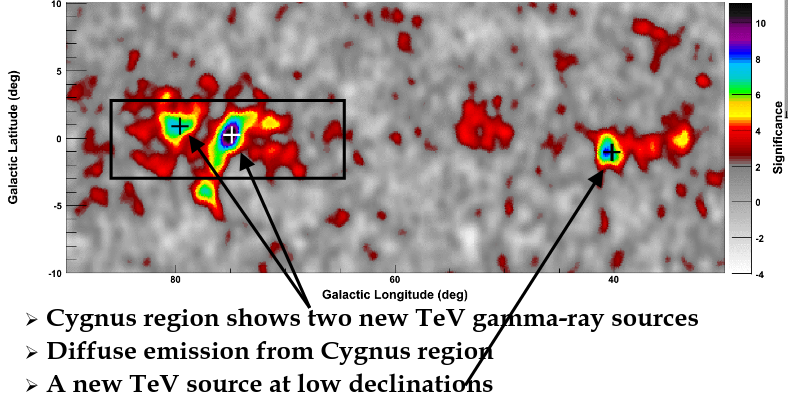
\includegraphics[width=0.8\textwidth]{figures/milagro_6.png}
\caption{\label{fig:x4} Milagro: a gamma-ray observatory in Los Alamos, NM.  Pictured: Cygnus Region.}
\end{figure}
\end{frame}

\begin{frame}{Who detects them?}
\begin{figure}
\centering
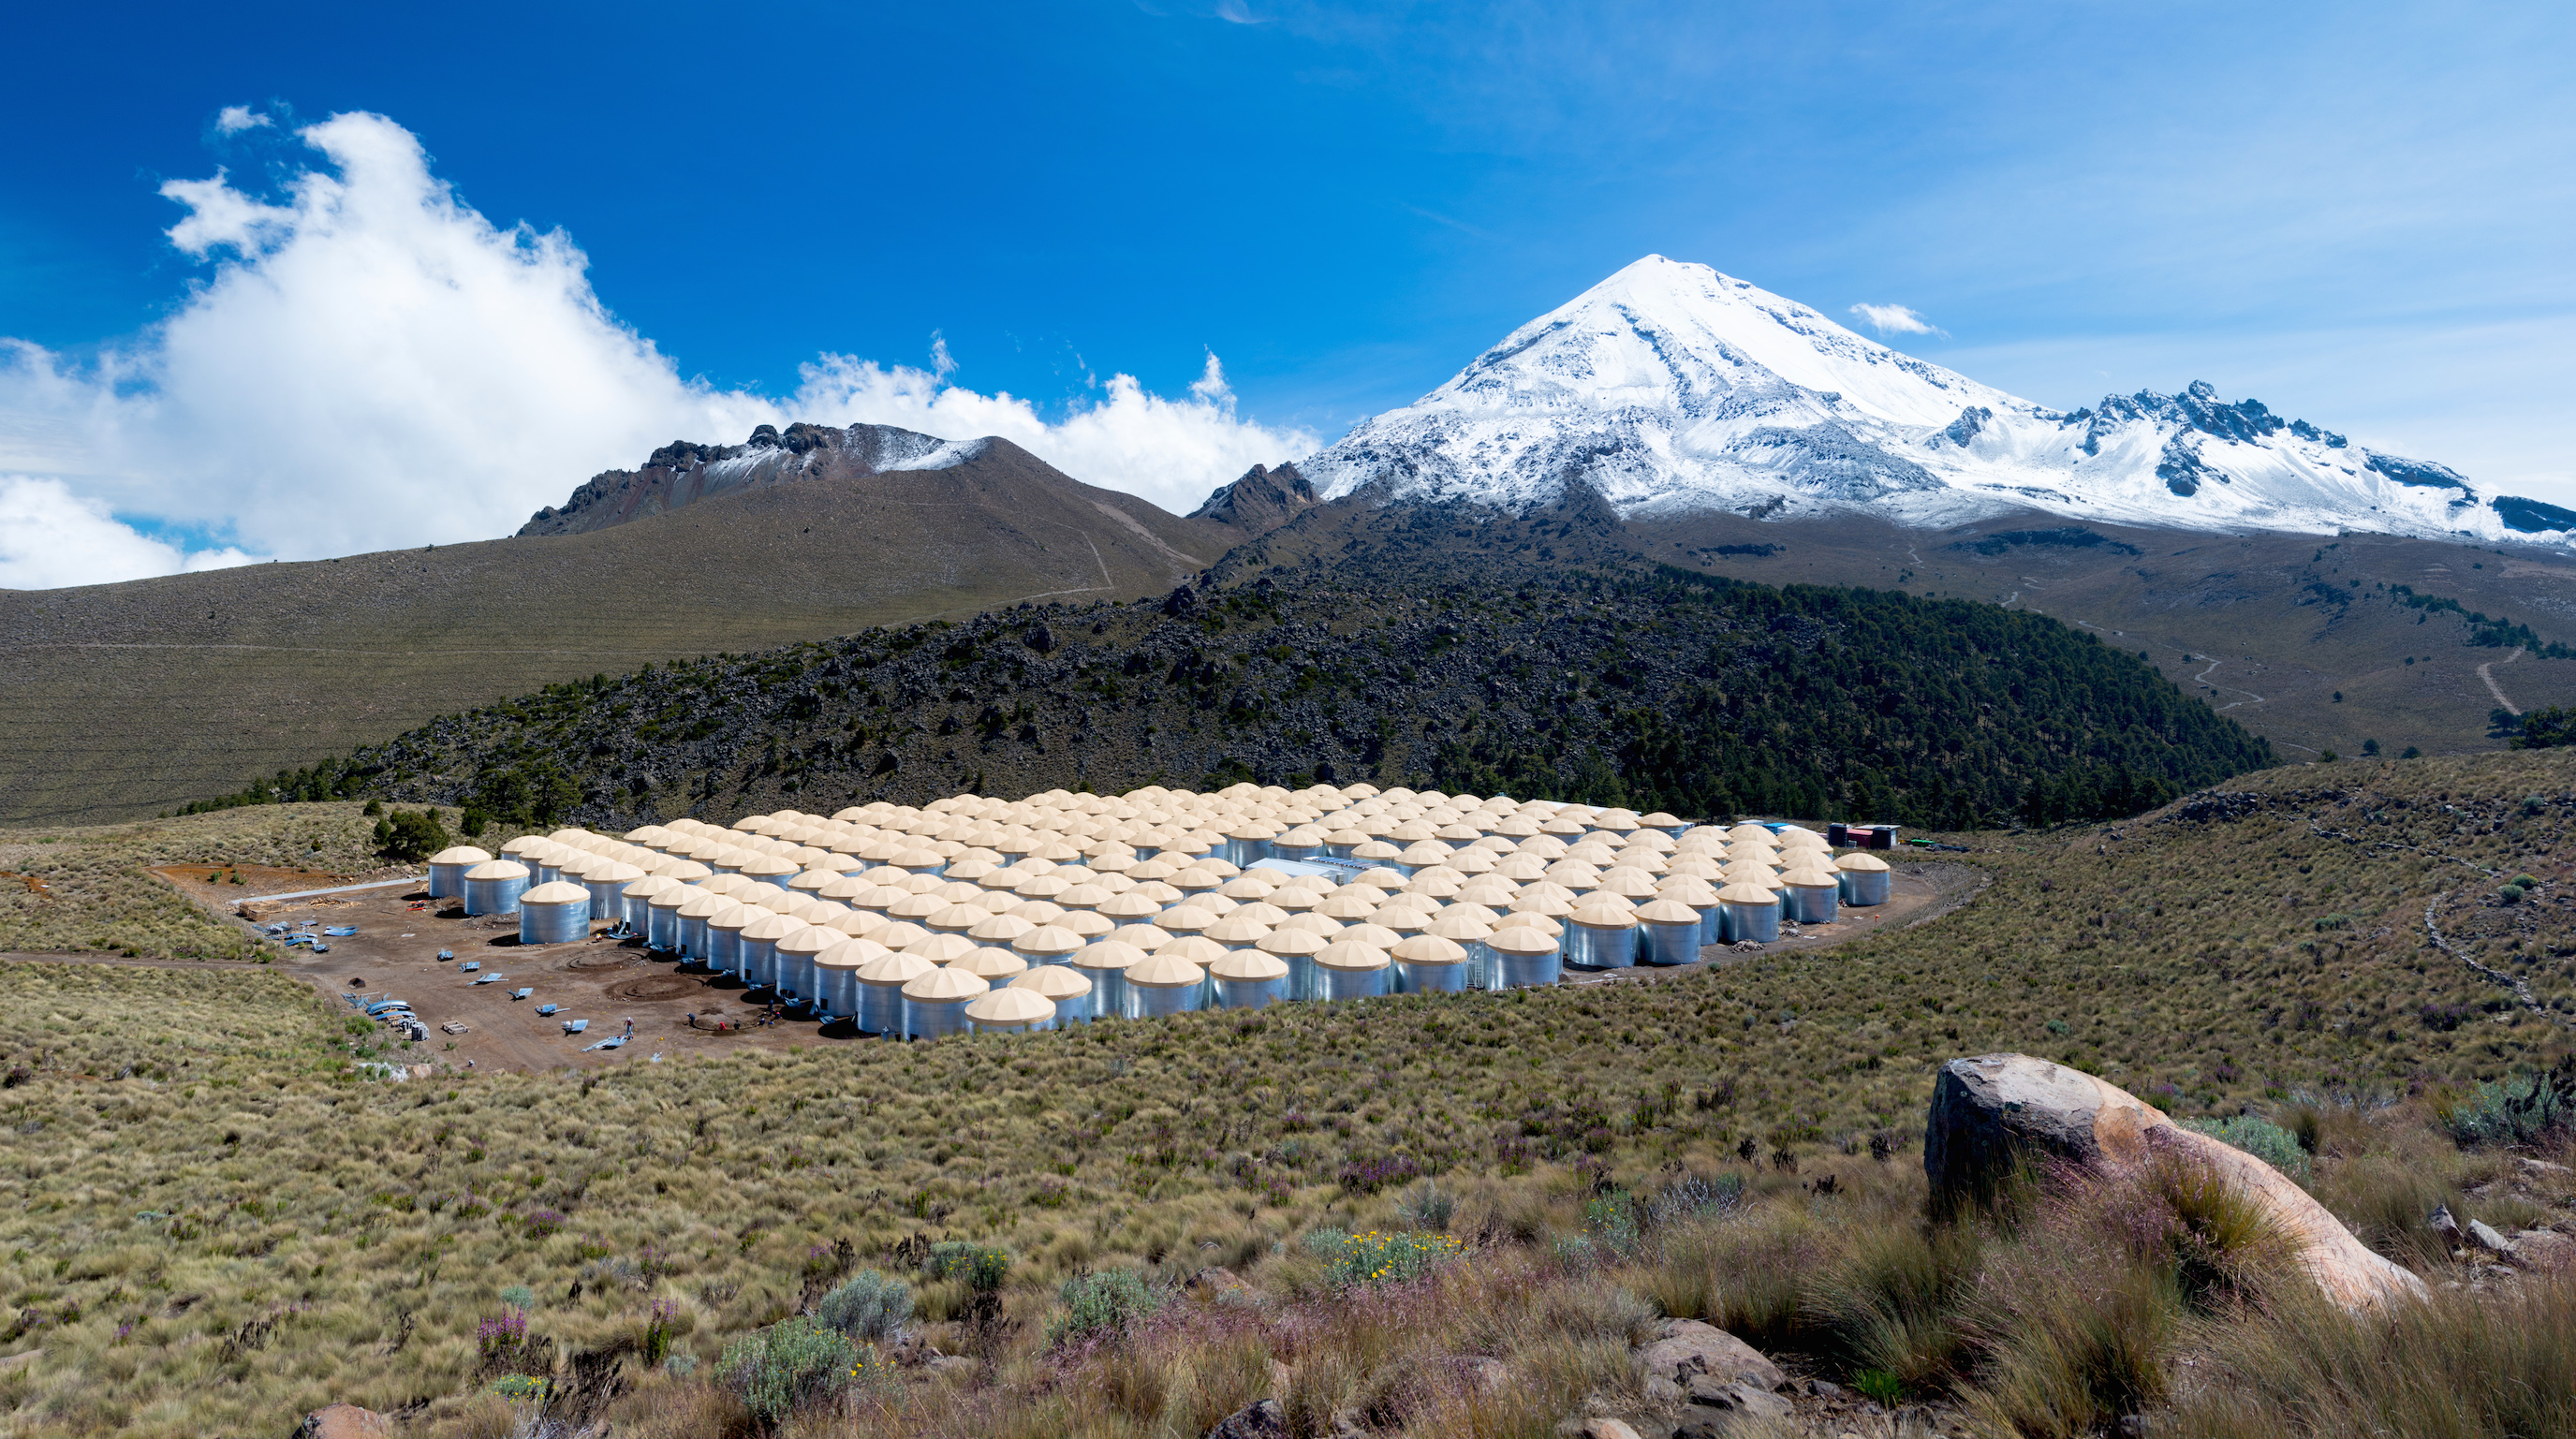
\includegraphics[width=0.8\textwidth]{figures/hawc_1.jpg}
\caption{\label{fig:y1} HAWC: High Altitude Water Cherenkov detector.}
\end{figure}
\end{frame}

\begin{frame}{Who detects them?}
\begin{figure}
\centering
\includegraphics[width=0.5\textwidth]{figures/hawc_2.jpg}
\caption{\label{fig:y2} HAWC: High Altitude Water Cherenkov detector.}
\end{figure}
\end{frame}

\begin{frame}{Who detects them?}
\begin{figure}
\centering
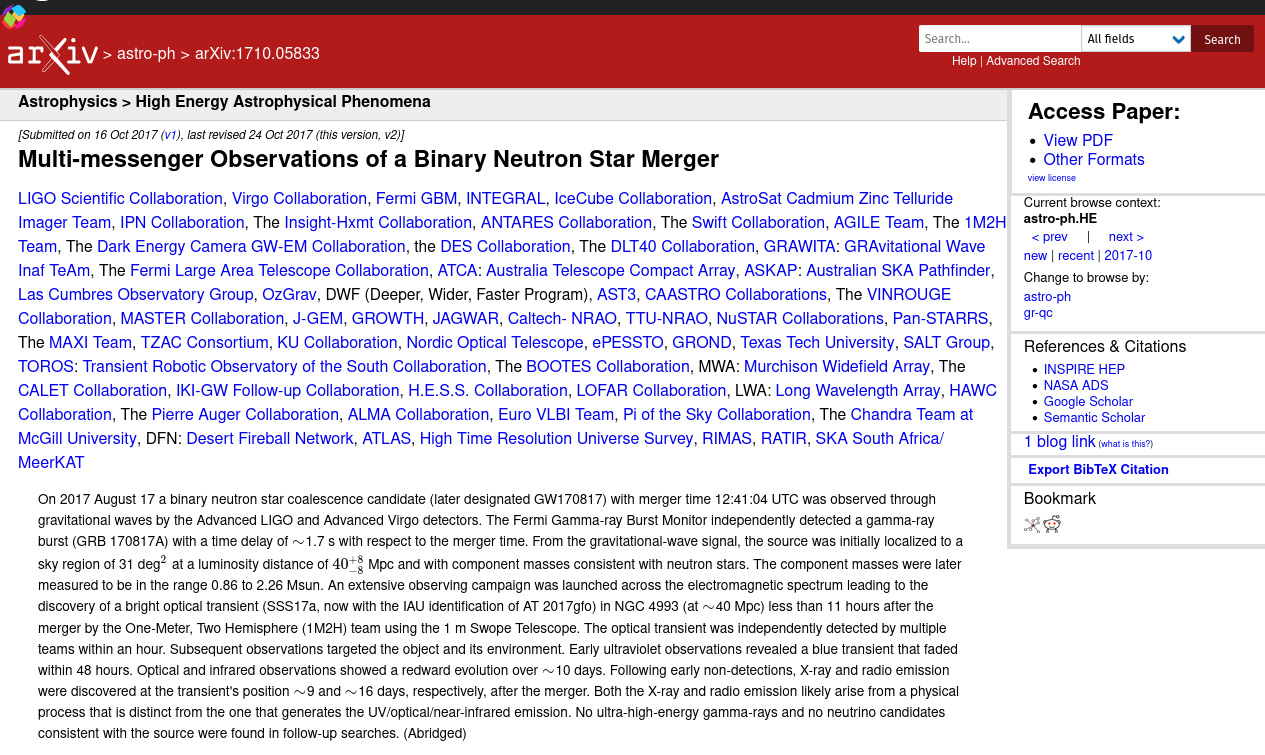
\includegraphics[width=0.4\textwidth]{figures/hawc_5.png}
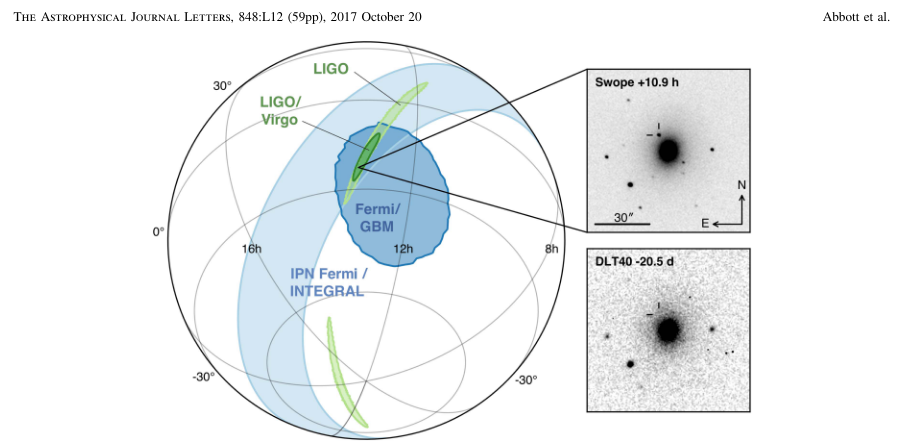
\includegraphics[width=0.55\textwidth]{figures/hawc_6.png}
\caption{\label{fig:y3} HAWC: High Altitude Water Cherenkov detector.}
\end{figure}
\end{frame}

\begin{frame}{Who detects them?}
\begin{figure}
\centering
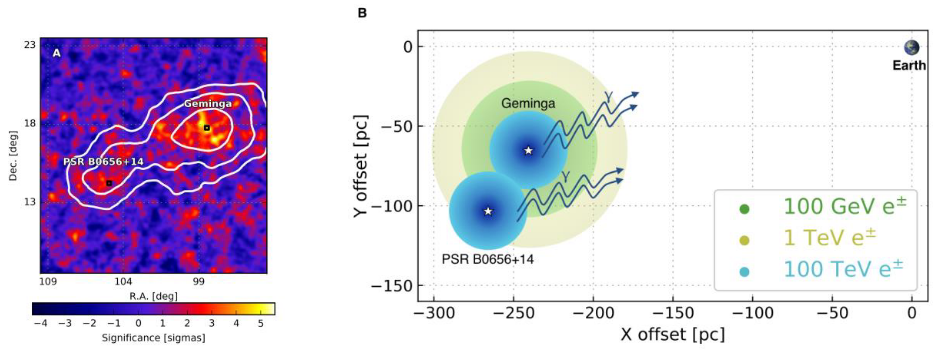
\includegraphics[width=0.6\textwidth]{figures/hawc_7.png}
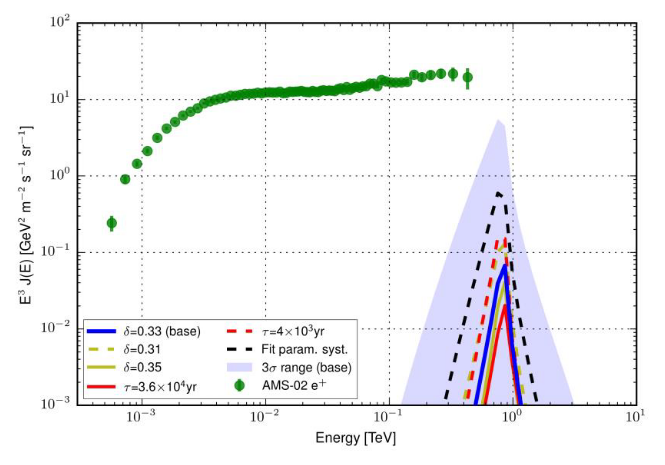
\includegraphics[width=0.35\textwidth]{figures/hawc_8.png}
\caption{\label{fig:y4} HAWC: High Altitude Water Cherenkov detector.}
\end{figure}
\end{frame}

\begin{frame}{SWGO: Southern Wide Field Gamma-ray Observatory}
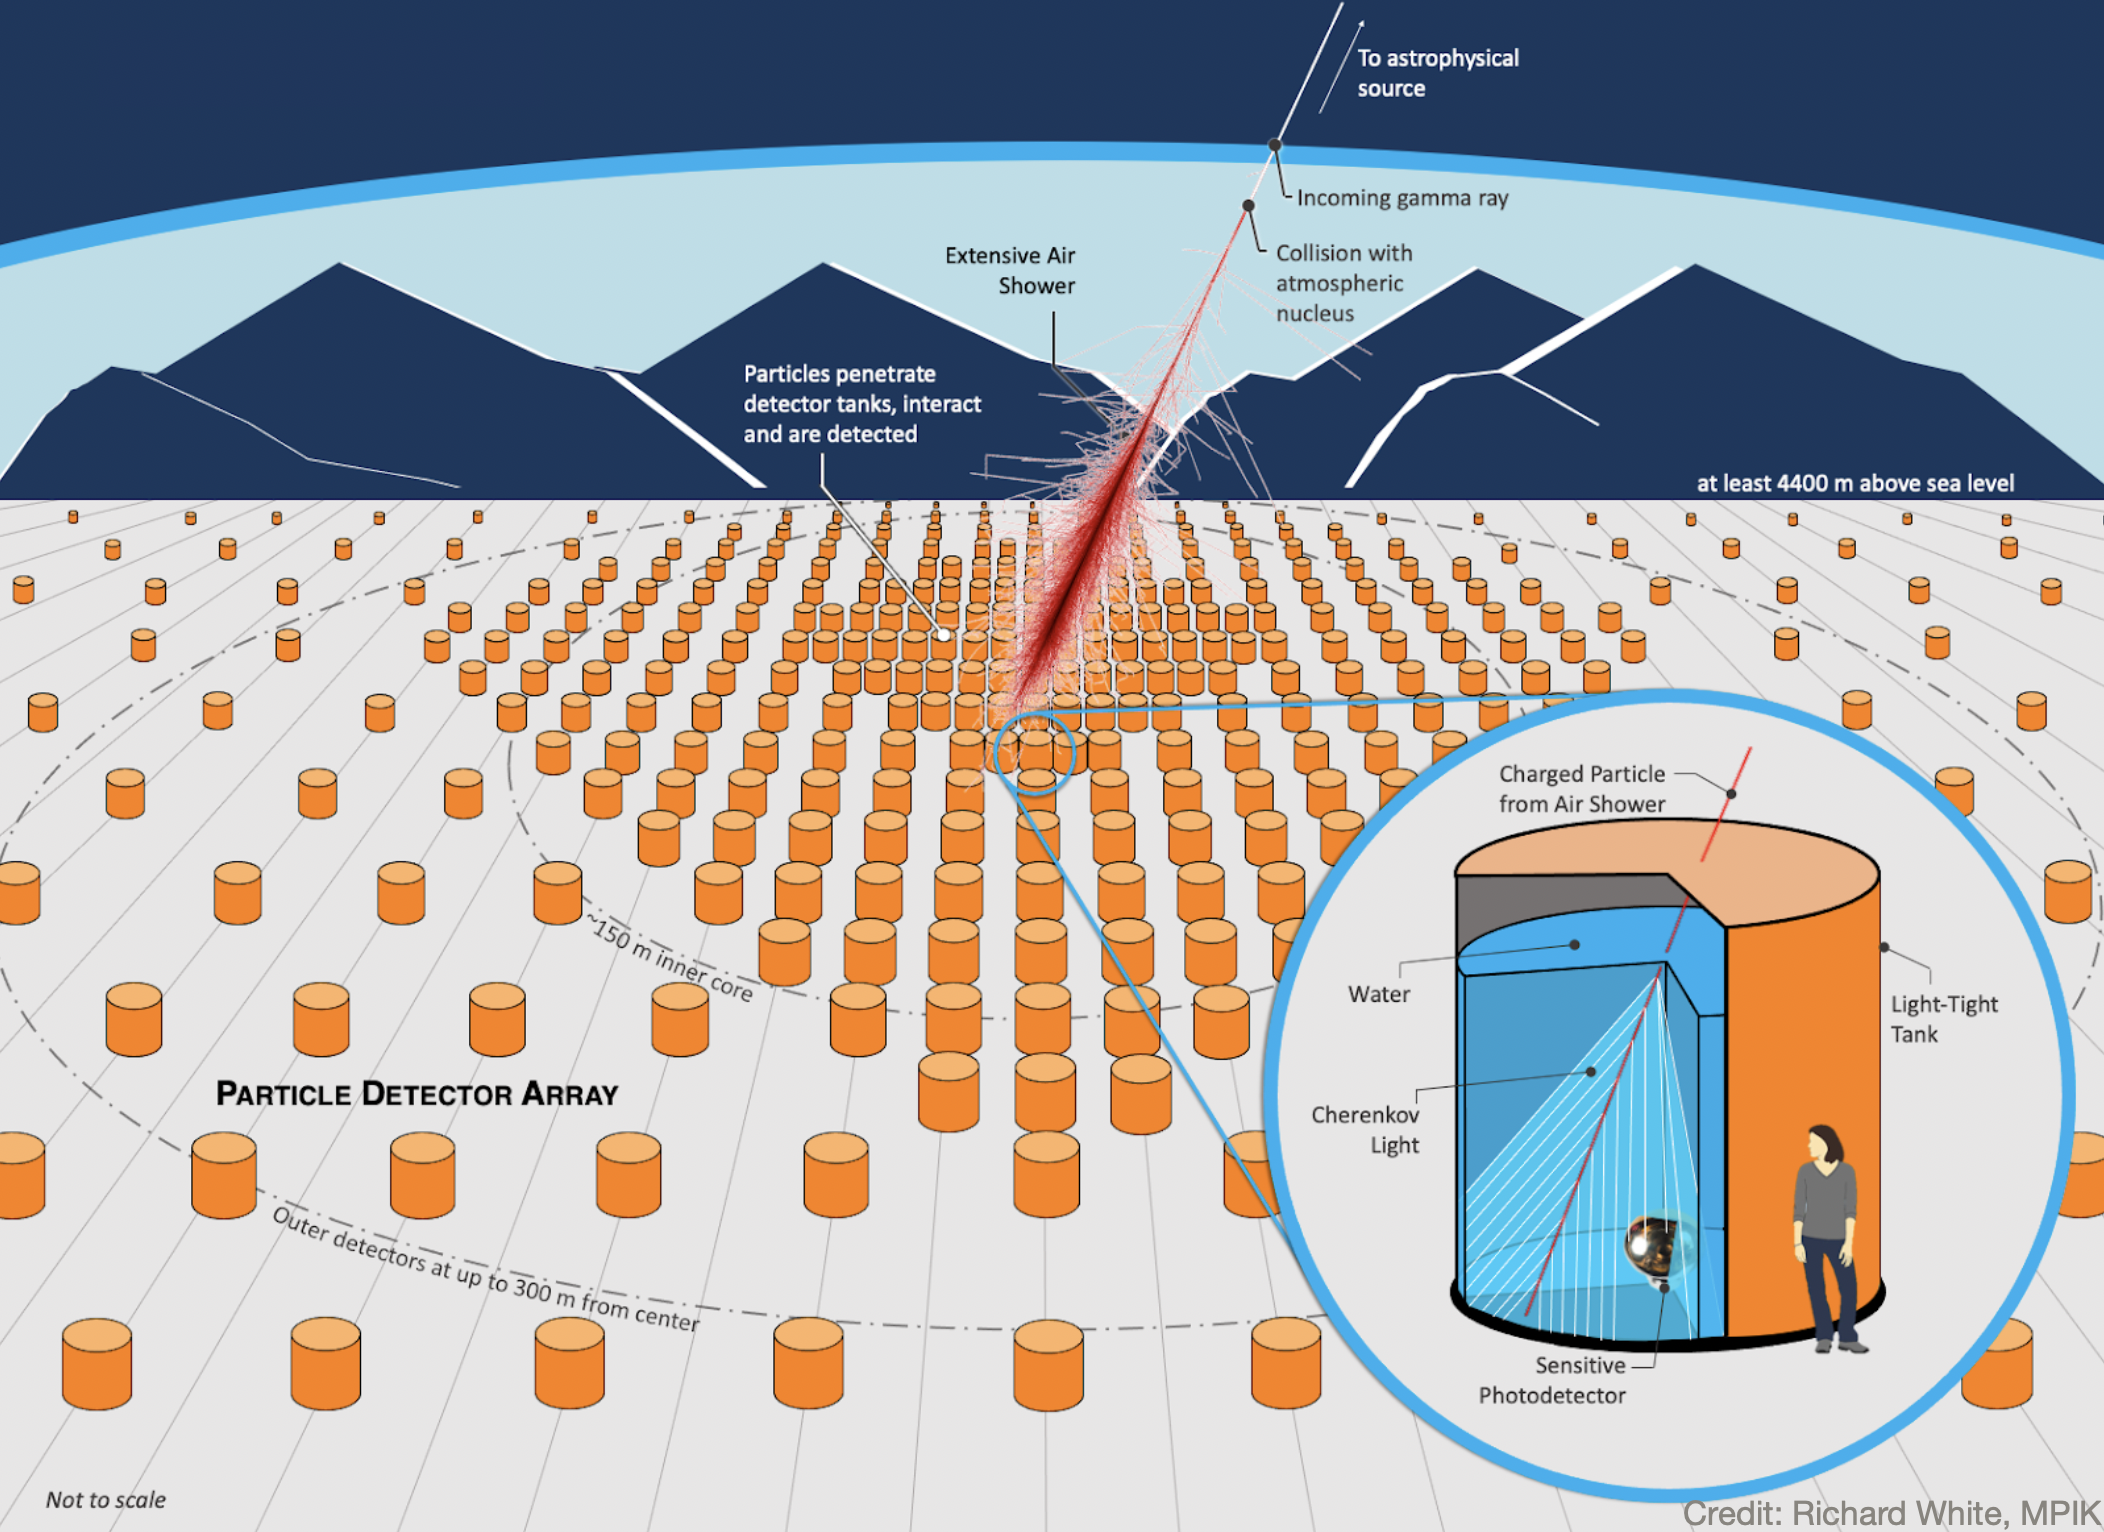
\includegraphics[width=\textwidth]{figures/swgo_1.png}
\end{frame}

\section{Conclusion}

\begin{frame}{Introduction: Gamma Ray Astrophysics}
\begin{enumerate}
\item \textbf{What is a high-energy gamma ray?}
\begin{itemize}
\item Units of energy
\item Types of particles
\item Air showers
\item Astrophysical sources
\end{itemize}
\item \textbf{How do we detect them?}
\begin{itemize}
\item The Cherenkov effect in water
\item Water-based detectors and photo-multiplier tubes (PMTs)
\end{itemize}
\item \textbf{Who detects them?}
\begin{itemize}
\item International collaborations of scientists
\item Detectors located in New Mexico, Mexico, and Chile
\end{itemize}
\end{enumerate}
\end{frame}

\end{document}